\documentclass[simplex.tex]{subfiles}
\definecolor{jgreen}{HTML}{197300}
\definecolor{jblue}{HTML}{0000cd}
\definecolor{jred}{HTML}{cc0000}
% NO NEED TO INPUT PREAMBLES HERE
% packages are inherited; you can compile this on its own
\definecolor{jgreen}{HTML}{197300}
\definecolor{jblue}{HTML}{0000cd}
\definecolor{jred}{HTML}{cc0000}
\begin{document}
\subsection[meda]{meda \href{https://github.com/mrae}{@JesseLP}}

%% April

Some timing tests were conducted to determine which methods/functions
contribute the most to processing time, see figure
\ref{fig:medaTimeTest}.  The figure implies that attention should be
given to \verb+Hgmm+ which is our current implmentation of hierarchical
Gaussian mixture models. 
Other work on MEDA this month has been mostly devoted to creating a docker
container and shifting the code base to be cloud friendly. 
A development version is  now available on
\href{https://hub.docker.com/r/neurodata/meda/}{Docker Hub}.  
This will allow processing of data with meda to be deployed in the cloud.  


\begin{figure}[!h]
\begin{cframed}
\centering
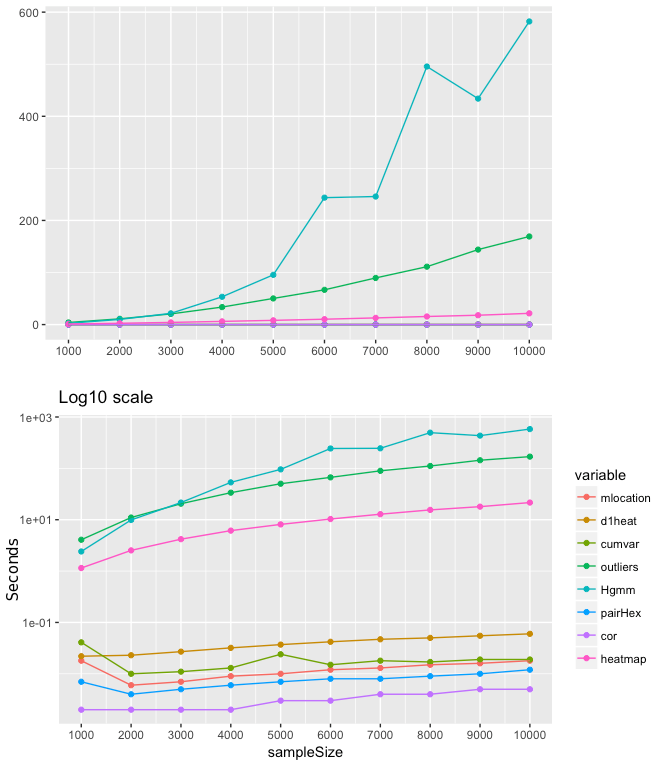
\includegraphics[width=0.6\textwidth]{../../figs/medaTimeTest.png}
\caption{Timing plots for the functions used in meda.  The bottom plot
  is the log scale of the top one. The data used consisted of 10,000
  observations in 24 dimensions, sampled in chunks of inceasing size.
  The Hgmm function takes about 10 minutes  on the largest sample used.}
\label{fig:medaTimeTest}
\end{cframed}
\end{figure}





\clearpage

\end{document}
